\documentclass[aspectratio=169]{beamer}
\usepackage[utf8]{inputenc}
\usepackage{utopia} %font utopia imported
\usetheme{Madrid}
\usecolortheme{default}
\usepackage{pgfplots}
\usepackage{tikz}

\usepackage{tikz-3dplot} 
\usepackage[european resistor, european voltage, european current]{circuitikz}
\usetikzlibrary{arrows,shapes,positioning}
\usetikzlibrary{decorations.markings,decorations.pathmorphing,
decorations.pathreplacing}
\usetikzlibrary{calc,patterns,shapes.geometric}

%Information to be included in the title page:
\title{Cours d'introduction à la chimie quantique}

\subtitle{Chapitre 3 : Cas simple\\Partie 3 : Particule libre sur une sphère}
\author{François Dion}
%\institute{Overleaf}
\date{2020}




%\logo{\includegraphics[height=1.5cm]{lion-logo.jpg}}

%End of title page configuration block
%------------------------------------------------------------



%------------------------------------------------------------
%The next block of commands puts the table of contents at the 
%beginning of each section and highlights the current section:

%\AtBeginSection[]
%{
  %\begin{frame}
    %\frametitle{Table of Contents}
    %\tableofcontents[currentsection]
  %\end{frame}
%}
%------------------------------------------------------------


\begin{document}

%The next statement creates the title page.
\frame{\titlepage}


%---------------------------------------------------------
%This block of code is for the table of contents after
%the title page
%\begin{frame}
%\frametitle{Table of Contents}
%\tableofcontents
%\end{frame}
%---------------------------------------------------------


\section{1er cas : Particule sur un cercle}
\begin{frame}
\frametitle{Le système}
Considérons le cas ou le potentiel est nul sur une cerlce, mais infini partout ailleur. La particule est restreinte à tourner sur un cercle de rayon $\vec{r}$ 
\begin{figure}
\tdplotsetmaincoords{75}{50} % to reset previous setting
\begin{tikzpicture}[scale=2.7,tdplot_main_coords,rotate around x=90]
 
  % variables
  \def\rvec{1.2}
  \def\thetavec{40}
  \def\phivec{70}
  \def\R{1.1}
  \def\w{0.3}
 
  % axes
  \coordinate (O) at (0,0,0);
  \draw[thick,->] (1,0,0) -- (2.5,0,0) node[below left]{$x$};
  \draw[thick,->] (1,0,0) -- (1,1,0) node[below right]{$z$};
  \draw[thick,->] (1,0,0) -- (1,0,1.4) node[below right]{$y$};
  \filldraw (1.6,0,1) circle (1pt);
 
 
  % circle - LHC
  \tdplotdrawarc[thick,rotate around x=90,black!70!blue]{(\R,0,0)}{\R}{0}{360}{}{}
 
 
 
\end{tikzpicture}

\end{figure}
\end{frame}

\begin{frame}
\frametitle{Le système}
L'hamiltonien général d'un système conservatif bidimensionnel est

\begin{equation}
\hat{H}=-\frac{\hbar^2}{2m} \left( \frac{\partial^2}{x^2} + \frac{\partial^2}{y^2}\right)+\hat{V}
\end{equation}

Dans ce système, la particule ne peut se trouver que sur le cercle, o\'u le potentiel est nul. Le terme $\hat{V}$ est donc nul.
Les variables $x$ et $y$ peuvent se définir en fonction des variables $r$ et $\theta$

\begin{figure}
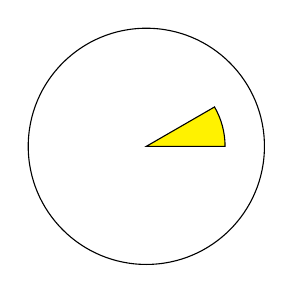
\begin{tikzpicture}
\draw (-4,0) circle (1.5cm);
 \filldraw[fill=yellow,draw=black] (-4,0) -- (-3,0) arc (0:30:1) -- cycle node[right] {$\thera$};
   
\end{tikzpicture}

\end{figure}
\end{frame}
\end{document}



